
% !TEX program = pdflatex
% !TEX enableSynctex = true
% !BIB program = bibtex

\documentclass[notes]{beamer}

%Cheat-Sheet: https://www.cpt.univ-mrs.fr/~masson/latex/Beamer-appearance-cheat-sheet.pdf
\usetheme{Frankfurt}

%-- Layout --%
% font size
\usepackage[fontsize=11pt]{scrextend}
\usepackage{amsmath}
\usepackage[short]{optidef}
\usepackage[backend=bibtex,style=authoryear]{biblatex}
% page
\setbeamersize{text margin left=1cm, text margin right=1cm}
\setbeamercolor{button}{bg=blue, fg=white}
% line space 
% footline
\addtobeamertemplate{navigation symbols}{}{
    \usebeamerfont{footline}
    % \usebeamercolor[fg]{footline}
    \hspace{2em}
    \insertframenumber/\inserttotalframenumber    }
% headline
\setbeamercovered{transparent}

%-- Figure --%
\usepackage{graphicx}
% \usepackage{subfig}

%-- Table --%
\usepackage{tabularx,booktabs}
\newcolumntype{Y}{>{\centering\arraybackslash}X}

%-- Text --%
\usepackage{xcolor}
% \usepackage{tikz}

%-- Math --%
\usepackage{amssymb}
\usepackage{amsmath}

%-- Caption --%
\usepackage{caption}
\usepackage{subcaption}

%-- Effects --%
\usepackage{hyperref}

%----------------------------------------------------------------------------------------
%	TITLE PAGE
%----------------------------------------------------------------------------------------

\title[]{The Nature of Corporate Credit Constraints} % The short title appears at the bottom of every slide, the full title is only on the title page

\author{Barnab\'as Sz\'ekely} % Your name

\date{\today } % Date, can be changed to a custom date

\begin{document}
\renewcommand{\arraystretch}{1.4}

\begin{frame}
\titlepage % Print the title page as the first slide
\end{frame}

%%----------------------------------------------------------------------------------------
%	PRESENTATION SLIDES
%----------------------------------------------------------------------------------------

%------------------------------------------------
\section{Intro}

\begin{frame}[label=slide2]
\frametitle{Asset-Based and Cash Flow-Based lending}
Asset based lending 
\begin{itemize}
 \setlength\itemsep{0em}
    \item secured against physical assets, in-default payments are expected from liquidation of the collateral
    \item implies asset-based constraints $\rightarrow$ traditional approach
\end{itemize} 
Cash flow-based lending
\begin{itemize}
 \setlength\itemsep{0em}
    \item not secured against any specific assets, in-default payments are expected from reorganization 
    \item approx. 75\% of total debt by volume! 
    \item implies earnings-based borrowing constraints
\end{itemize} \vspace{3mm}
Reconsider the effects of credit frictions: Lian and Ma (2021), Dreschel (2023), Greenwald (2019), Choi (2023) etc.
\end{frame}

%------------------------------------------------
\begin{frame}[label=slide2]
\frametitle{Data and Motivation}
Compustat and Capital IQ data; US traded firms; 2010-2023
\begin{table}[h!]
\centering
\resizebox{0.85\textwidth}{!}{% 0.75 times the text width
\begin{tabular}{l|rrr}
\multicolumn{4}{l}{\textbf{Firm shares by debt financing strategy}} \\
\toprule
\textbf{Share by} & \textbf{\# of Firms} & \textbf{Assets}  & \textbf{Borrowing} \\  
Asset-based borrowers & 35.66\% & 4.83\% & 3.36\% \\ 
'Hybrid' borrowers & 52.11\% & 87.27\% & 90.31\% \\ 
CF-based borrowers & 12.23\% & 7.91\% & 6.33\% \\ 
\bottomrule
\end{tabular}
}
\label{tab:shares}
\end{table}
\textbf{Takeaway}: most firms rely on both type of debt - considering ABL vs. CFL borrowers misses this fact!

\end{frame}

%------------------------------------------------
\begin{frame}
  \frametitle{Research question}
  
So are asset-based or earnings based constraints more relevant? 
\begin{itemize}
    \item Neither! Most firms face a combination of the two
\end{itemize} \vspace{5mm} \\
I explore credit frictions along these lines: 
\begin{itemize}
 \setlength\itemsep{0em}
    \item Empirical: the determinants of firms' debt financing strategies
    \item Structural: precise description of credit frictions and their aggregate implications
\end{itemize}
  

\end{frame}
%------------------------------------------------
\section{Evidence}

\begin{frame}
  \frametitle{Empirical analysis - CFL reliance}

  \begin{columns}
    \begin{column}{0.55\textwidth} % Adjust the width as needed
    
    $ CFL \ reliance = CFL \ debt / Total \  debt $ \vspace{1mm} \\

    The main determinants of CFL: 
    \begin{itemize}
     \setlength\itemsep{0em}
        \item Size (total assets)
        \item Leverage
        \item Asset pledgeability
    \end{itemize}
    Fixed costs of lending against future cash flows: 
    \begin{itemize}
        \setlength\itemsep{0em}
        \item High share of ABL only firms
        \item Smaller and less indebted
    \end{itemize}
    
 \end{column}
 \begin{column}{0.45\textwidth} % Adjust the width as needed
     \begin{figure}
        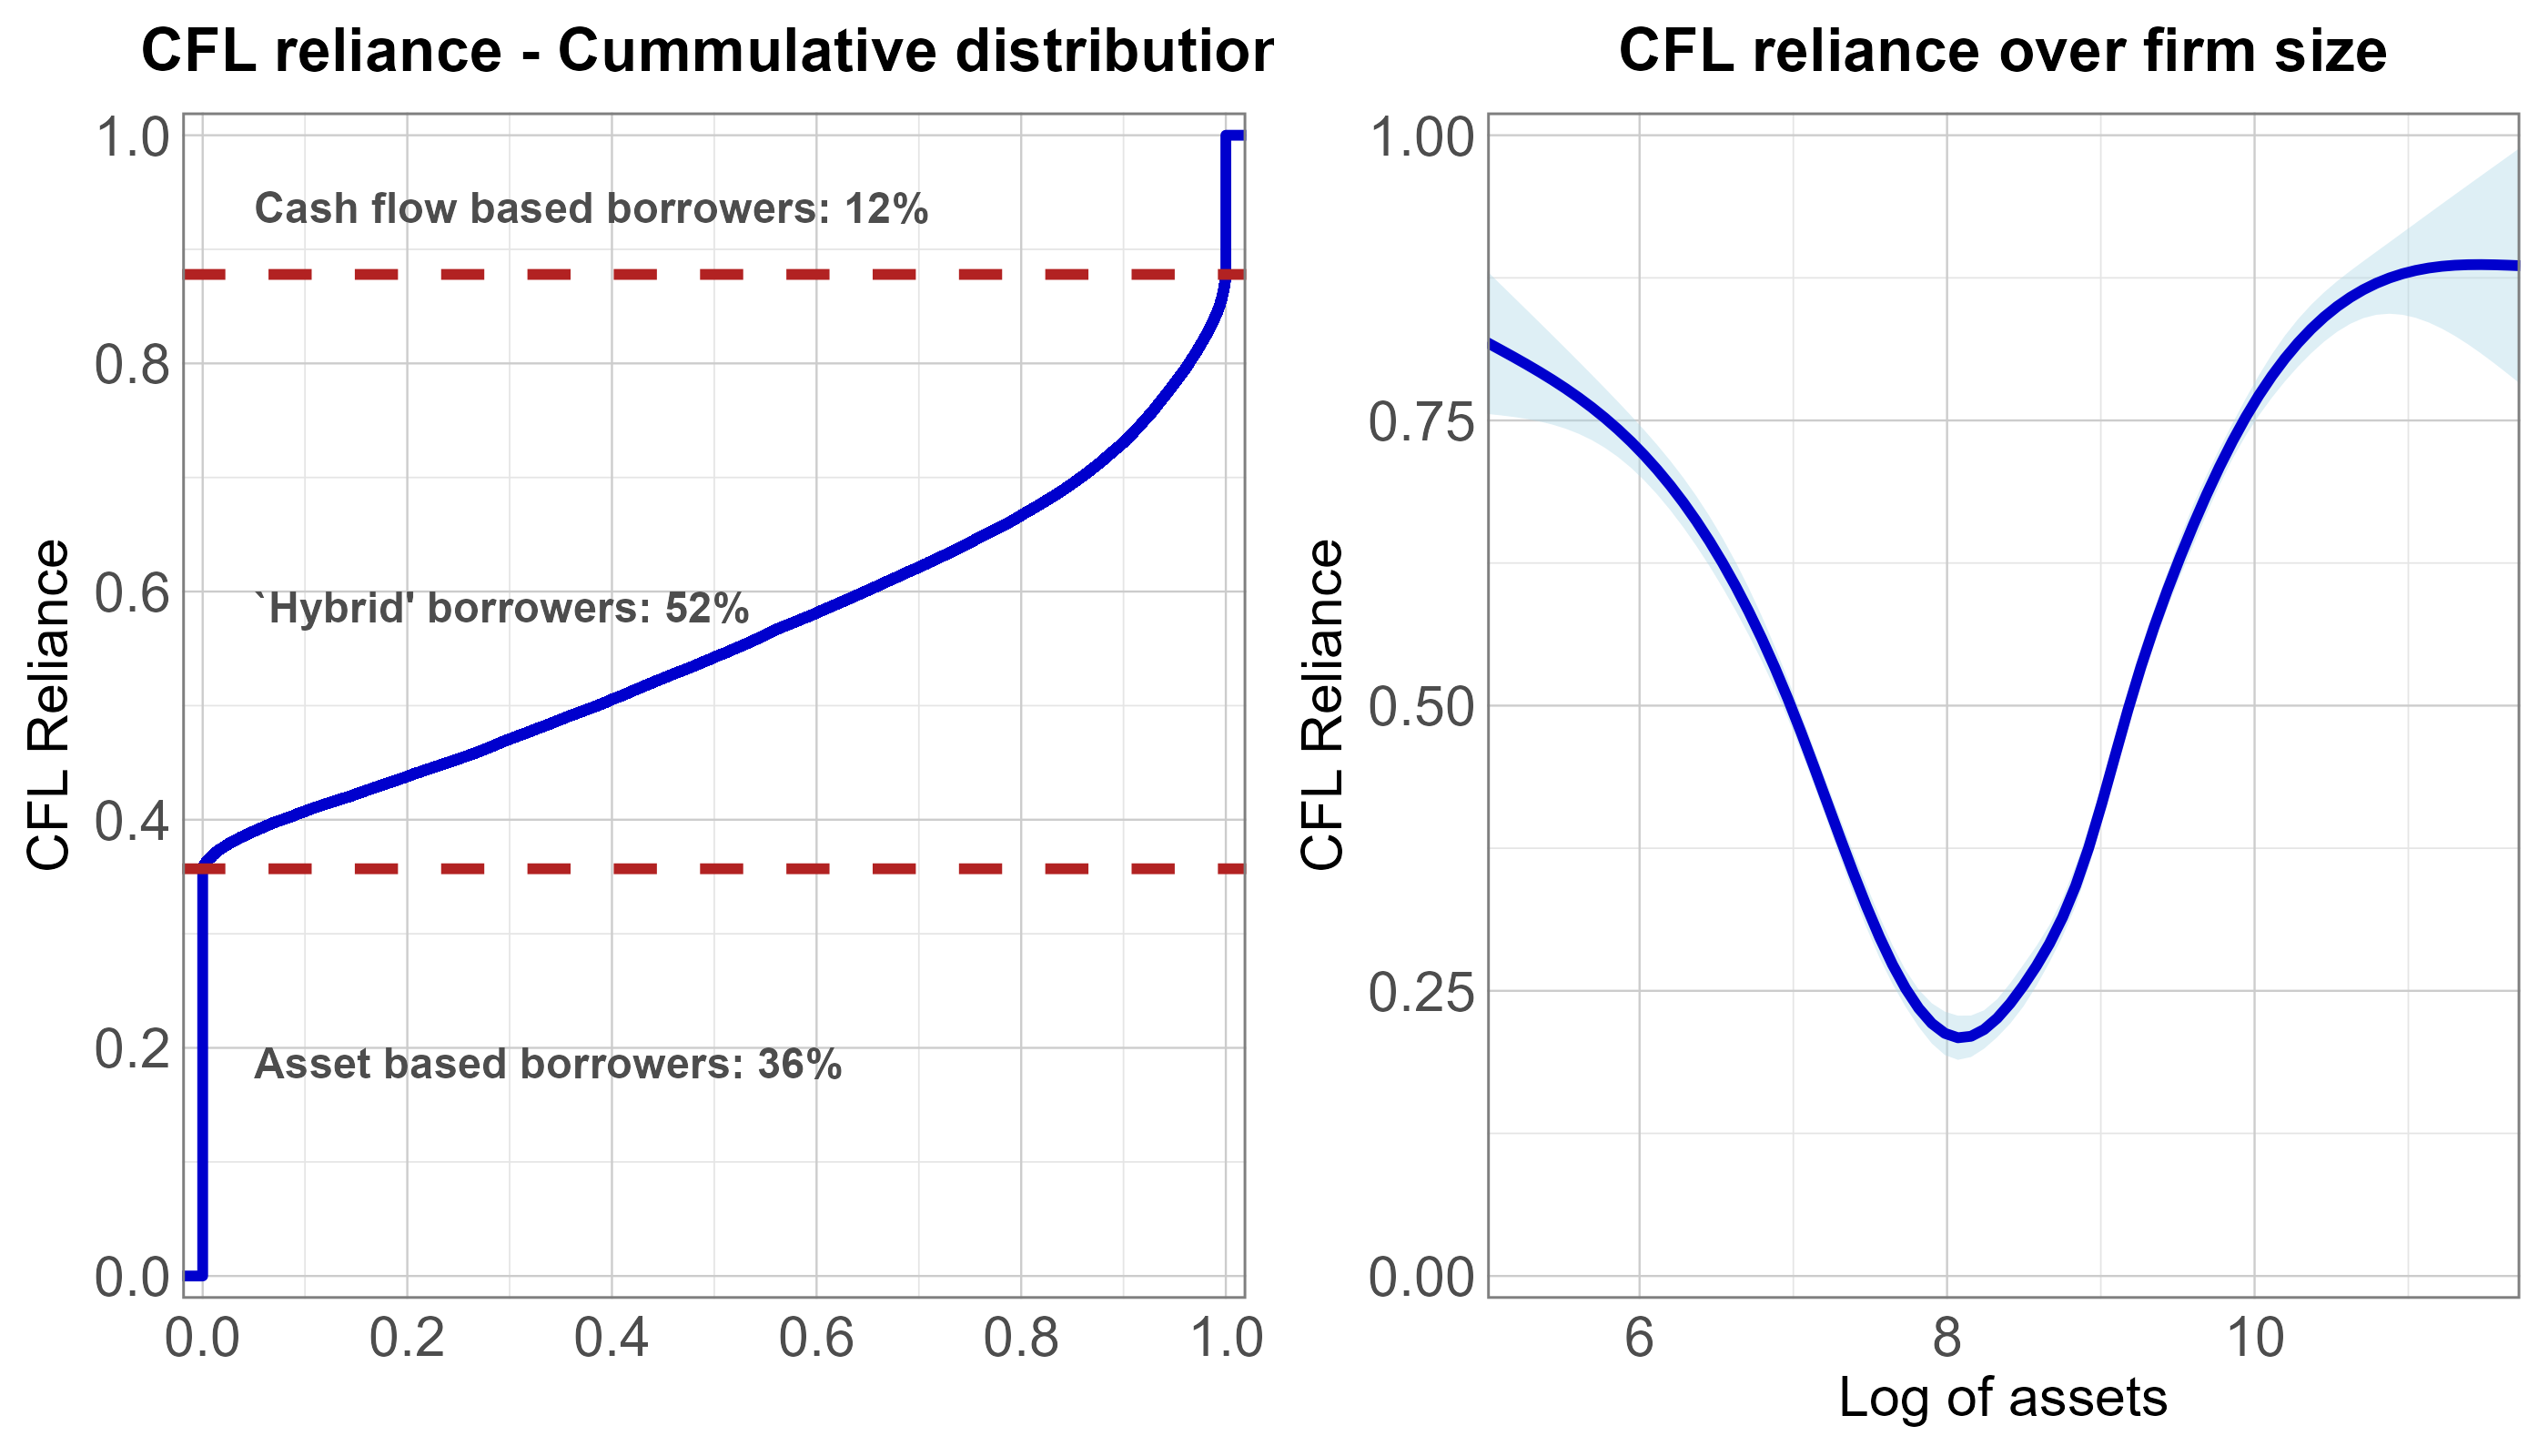
\includegraphics[width=\textwidth]{C:/Users/szjud/OneDrive/Asztali gép/EBCs/CFL-git/Latex codes/Plots/presentations/smoothcfd.png} % Adjust the path and options as needed
      \end{figure}
    \end{column}
  \end{columns}
\end{frame}

%------------------------------------------------
\begin{frame}[label=slide2]
\frametitle{Qualitative analysis - fixed costs}
In-default:  reorganization costs
\begin{itemize}
\item ABL: liquidation (Chapter 7)  $\rightarrow$ relatively quick and costless
\item CFL: reorganization (Chapter 11) $\rightarrow$ costly: negotiation between debtors and creditors, legal fees, time expense etc.
\end{itemize} \vspace{3mm}
No default: monitoring costs
\begin{itemize}
\item ABL: only a periodic appraisal of assets
\item CFL: lender must carry out `due diligence' on an ongoing basis
\end{itemize}
These explain why small firms may be shout out of cash flow-based debt financing

\end{frame}


\section{Model}

%------------------------------------------------
\begin{frame}[label=slide2]
\frametitle{Costs of borrowing: $q^{cfl}$ vs. $q^{abl}$}
\textbf{GE model}, cost of external finance from the zero profit condition \vspace{4mm} \\
\textbf{ABL}: the lender liquidates assets subject to a variable cost:
$$ q^{abl}(k',b')b' = \beta \left[ (1-P_\chi) b' + P_\chi \min\{b', \ \phi_k (1-\delta) k' \} \right]    $$ 
\textbf{CFL}: the lender takes over the entire firm and resells it to the household subject to a variable \textbf{and} fixed costs ($\zeta_1$ and $\zeta_2$)
\begin{equation*}
    \resizebox{1\hsize}{!}{$
    q^{cfl}(k',b',\varepsilon_i)b' = \beta \left[ (1-P_\chi) b' + P_\chi \sum_{j=1}^{N_\varepsilon} g_{ij}  \min\{b', \ V^D_1(k',b',\varepsilon_j')  \} - \zeta_2 \right]
    $}
\end{equation*}

where 
$$V_1^D(k,b,\varepsilon_i) = \max \Big\{ \phi_vV_2(k,b,\varepsilon_i)- \zeta_1, \  \phi_k (1-\delta) k - b \Big\}.$$
\end{frame}

\end{document}
